%\documentclass[draft]{beamer}
\documentclass[dvips, 11pt]{beamer}
\mode<presentation>{
  \usetheme{CambridgeUS}
  \setbeamercovered{transparent}
}
\usepackage[latin1]{inputenc}
\usepackage[T1]{fontenc}
\usepackage{lmodern}
\usepackage[italian]{babel}
%\usepackage[overlay,absolute]{textpos}
\usepackage{graphicx}
\usepackage{tikz}
\usetikzlibrary{shapes, chains, scopes, shadows, positioning, arrows, decorations.pathmorphing}
\usepackage{appendixnumberbeamer}

\colorlet{arancio}{yellow!20!red!20}
\colorlet{viola}{blue!10!red!5}

\tikzstyle{disp}=[rectangle, rounded corners=10pt, align=center, drop shadow, fill=blue!20, draw=black!50]
\tikzstyle{db}=[cylinder, align=center, aspect=0.2, drop shadow, shape border rotate=90, fill=yellow!20, draw=black!50]
\tikzstyle{rdf}=[cylinder, align=center, aspect=0.2, drop shadow, shape border rotate=90, fill=yellow!50!red!20, draw=black!50]
\tikzstyle{web}=[rectangle, rounded corners=2pt, align=center, drop shadow, fill=green!20, draw=black!50]
\tikzstyle{weblist}=[rectangle, rounded corners=2pt, align=center, double copy shadow, fill=green!20, draw=black!50]
\tikzstyle{file}=[chamfered rectangle, chamfered rectangle corners = north east, align=center, drop shadow, fill=black!20, draw=black!50]
\tikzstyle{filelist}=[chamfered rectangle, chamfered rectangle corners = north east, align=center, double copy shadow, fill=black!20, draw=black!50]
\tikzstyle{gaz}=[tape, align=center, drop shadow, shape border rotate=90, fill=blue!10, draw=black!50]
\tikzstyle{gate}=[rectangle, rounded corners=2pt, align=center, drop shadow, fill=red!20, draw=black!50]
\tikzstyle{app}=[ellipse, align=center, drop shadow, fill=red!20, draw=black!50]
\tikzstyle{esp}=[cloud, aspect=2, align=center, drop shadow, fill=blue!10, draw=black!50]
\tikzstyle{rdfc}=[rectangle, rounded corners=5pt, align=center, drop shadow, fill=yellow!50!red!20, draw=black!50]
\tikzstyle{rdfclist}=[rectangle, rounded corners=5pt, align=center, double copy shadow, fill=yellow!50!red!20, draw=black!50]
\tikzstyle{webapp}=[ellipse, align=center, drop shadow, fill=green!20, draw=black!50]
\tikzstyle{app2}=[rectangle, rounded corners=2pt, align=center, drop shadow, fill=red!20, draw=black!50]
\tikzstyle{app3}=[rectangle, rounded corners=2pt, align=center, drop shadow, fill=green!20, draw=black!50]
\tikzstyle{app4}=[rectangle, rounded corners=2pt, align=center, drop shadow, fill=arancio, draw=black!50]
\tikzstyle{tab}=[rounded rectangle, align=center, drop shadow, fill=blue!10, draw=black!50]
\tikzstyle{man}=[circle, align=center, drop shadow, fill=red!20, draw=black!50]
\tikzstyle{label}=[rectangle, align=center, rounded corners=2pt, fill=yellow!20]
\tikzstyle{round}=[circle, align=center, drop shadow, text width=0cm, fill=blue!20, draw=black!50]
\tikzstyle{choice}=[diamond, align=center, drop shadow, fill=blue!20, draw=black!50]
\tikzstyle{legenda}=[rectangle, rounded corners=2pt, align=center, drop shadow, fill=viola, draw=black!50]
\tikzstyle{legendait}=[text width=10pt, text depth=10pt]
\tikzstyle{legendalab}=[]

\tikzstyle{freccia}=[->, very thick, >=stealth', draw=black!80]
\tikzstyle{ufreccia}=[->, >=stealth', draw=black!80, double]
\tikzstyle{tfreccia}=[->, dash pattern=on 3pt off2pt, very thick, >=stealth', draw=black!80]
\tikzstyle{tufreccia}=[->, dash pattern=on 3pt off2pt, >=stealth', draw=black!80, double]
\tikzstyle{dfreccia}=[<->, very thick, >=stealth', draw=black!80]
\tikzstyle{dtfreccia}=[<->, dash pattern=on 3pt off2pt, very thick, >=stealth', draw=black!80]
\tikzstyle{nfreccia}=[ very thick, >=stealth', draw=black!80]
\tikzstyle{tnfreccia}=[dash pattern=on 3pt off2pt, very thick, >=stealth', draw=black!80]

\tikzstyle{point}=[coordinate]
\tikzstyle{vuoto}=[text width=0pt]

\tikzstyle{forshadow}=[rectangle, rounded corners=2pt, drop shadow, inner sep = 0pt]
\tikzstyle{sqltable}=[rectangle split, rounded corners=2pt, inner sep = 2pt, rectangle split part align={center, left}, rectangle split parts=#1, draw, rectangle split part fill={green!20, yellow!20}, draw=black!50]

\colorlet{umlTit}{green!20}
\colorlet{umlAtt}{yellow!20!red!20}
\colorlet{umlMet}{yellow!20}
\tikzstyle{umltable}=[rectangle split, rounded corners=2pt, inner sep = 2pt, rectangle split part align={center, left}, rectangle split parts=#1, draw, rectangle split part fill={umlTit, umlMet}, draw=black!50]


\tikzstyle{coda}=[rectangle split, rectangle split part align={center}, rectangle split parts=#1, draw, fill=yellow!20, draw=black!50, drop shadow]

\tikzstyle{uri}=[ellipse, drop shadow, draw=black!50, fill=green!20, very thick]
\tikzstyle{letterale}=[rectangle, drop shadow, rounded corners=2pt, draw=black!50, fill=yellow!20, very thick]
\tikzstyle{arcol}=[->, >=stealth, draw=black!80, very thick, bend right]
\tikzstyle{labell}=[rectangle, rounded corners=2pt, fill=yellow!20, swap]
\tikzstyle{arcor}=[->, >=stealth, draw=black!80, very thick, bend left]
\tikzstyle{labelr}=[rectangle, rounded corners=2pt, fill=yellow!20]

\tikzstyle{uriEsistente}=[ellipse, drop shadow, draw=black!50, fill=blue!10, very thick]
\tikzstyle{uriChoice}=[rectangle, rounded corners=2pt, drop shadow, draw=black!50, fill=blue!10, very thick, align=left]

\tikzstyle{labelg}=[rectangle, rounded corners=2pt, sloped, above]%, fill=yellow!20]
\tikzstyle{labelog}=[rectangle, rounded corners=2pt, right]%, fill=yellow!20]

\tikzstyle{tempLab}=[rectangle, rounded corners=2pt, text width = 1.5cm, text height = 0.5cm, text depth = 0.25cm, align=center, drop shadow, fill=viola, draw=black!50]
\tikzstyle{tempLab2}=[rectangle, rounded corners=2pt, text width = 2cm, text height = 0.5cm, text depth = 0.25cm, align=center, drop shadow, fill=viola, draw=black!50]
\tikzstyle{tempLab3}=[rectangle, rounded corners=2pt, text width = 2cm, text height = 0.5cm, text depth = 0.75cm, align=center, drop shadow, fill=viola, draw=black!50]
\tikzstyle{tempHid3}=[rectangle, rounded corners=2pt, text width = 2cm, text height = 0.5cm, text depth = 0.75cm ]
\tikzstyle{tempLine}=[very thick, draw=black!80]
\tikzstyle{tempTLine}=[dash pattern=on 3pt off2pt, very thick, draw=black!80]
\tikzstyle{tempLineProc}=[very thick, draw=red!80]

\tikzstyle{evidenzia}=[draw opacity = 0.5, line width = 5pt, color=red, decorate, decoration={random steps,segment length=3pt,amplitude=1pt}]
\tikzstyle{evidenziaRett}=[evidenzia, draw]%, rounded corners = 5pt]
%\tikzstyle{evidenziaFrecc}=[draw opacity = 0.5, line width = 5pt, color=red, ->]
\tikzstyle{evidenziaFrecc}=[line width = 5pt, draw=red!50, decorate, decoration={random steps,segment length=3pt,amplitude=0.2pt}, ->]

\newcommand{\unicocodet}[1]{\texttt{\bfseries #1}}
\newcommand{\dimg}{\scriptsize}

\newcommand{\dimt}{\tiny}
\newcommand{\codt}[1]{\dimt #1}
%\newcommand{\codt}[1]{\dimt \unicocodet{#1}}


\title[Analisi e sviluppo di un crawler]{\textbf{\uppercase{Analisi e sviluppo di un crawler per la creazione di una base di conoscenza semantica del personale universitario}}}
\subtitle{parte del progetto OSIM (\emph{Open Space Innovative Minds})
  del DISIT (\emph{Distributed Systems and Internet Technology Laboratory}) della facolt\`a di ingegneria}
\institute[Universit\`a Firenze]{UNIVERSIT\`A DEGLI STUDI DI FIRENZE\\Facolt\`a di Scienze Matematiche, Fisiche e Naturali\\Corso di Laurea in Informatica}
  %\\ 
\includegraphics[width=2cm]{img/logo-unifi.eps}
\author[Stefano Martina]{
  \textbf{\uppercase{Stefano Martina}}\\
  Relatore: Elena Barcucci; Corelatore: Paolo Nesi
}

\date[20 luglio 2012]{Tesi di laurea, 20 luglio 2012}

\begin{document}

\begin{frame}
  \titlepage
\end{frame}

%\begin{frame}
%  \tableofcontents
  % You might wish to add the option [pausesections]
%\end{frame}

\section{Analisi del problema}

\subsection{Progetto OSIM}

\begin{frame}{Problematiche}
  \begin{itemize}
  \item I sistemi classici di ricerca non sono efficaci per certi ambiti
    \pause
  \item \`E necessaria la possibilit\`a di poter ricercare chi ha certe \alert{competenze}
    \pause
  \item Le pagine delle persone hanno una struttura \alert{complessa} e non semantica
    \pause
  \item \`E necessario fornire un'interfaccia sia per interrogare\\
    che per amministrare le competenze
  \end{itemize}
\end{frame}

\begin{frame}{Il progetto}
  \begin{block}{Schema di OSIM}
    \begin{center}
      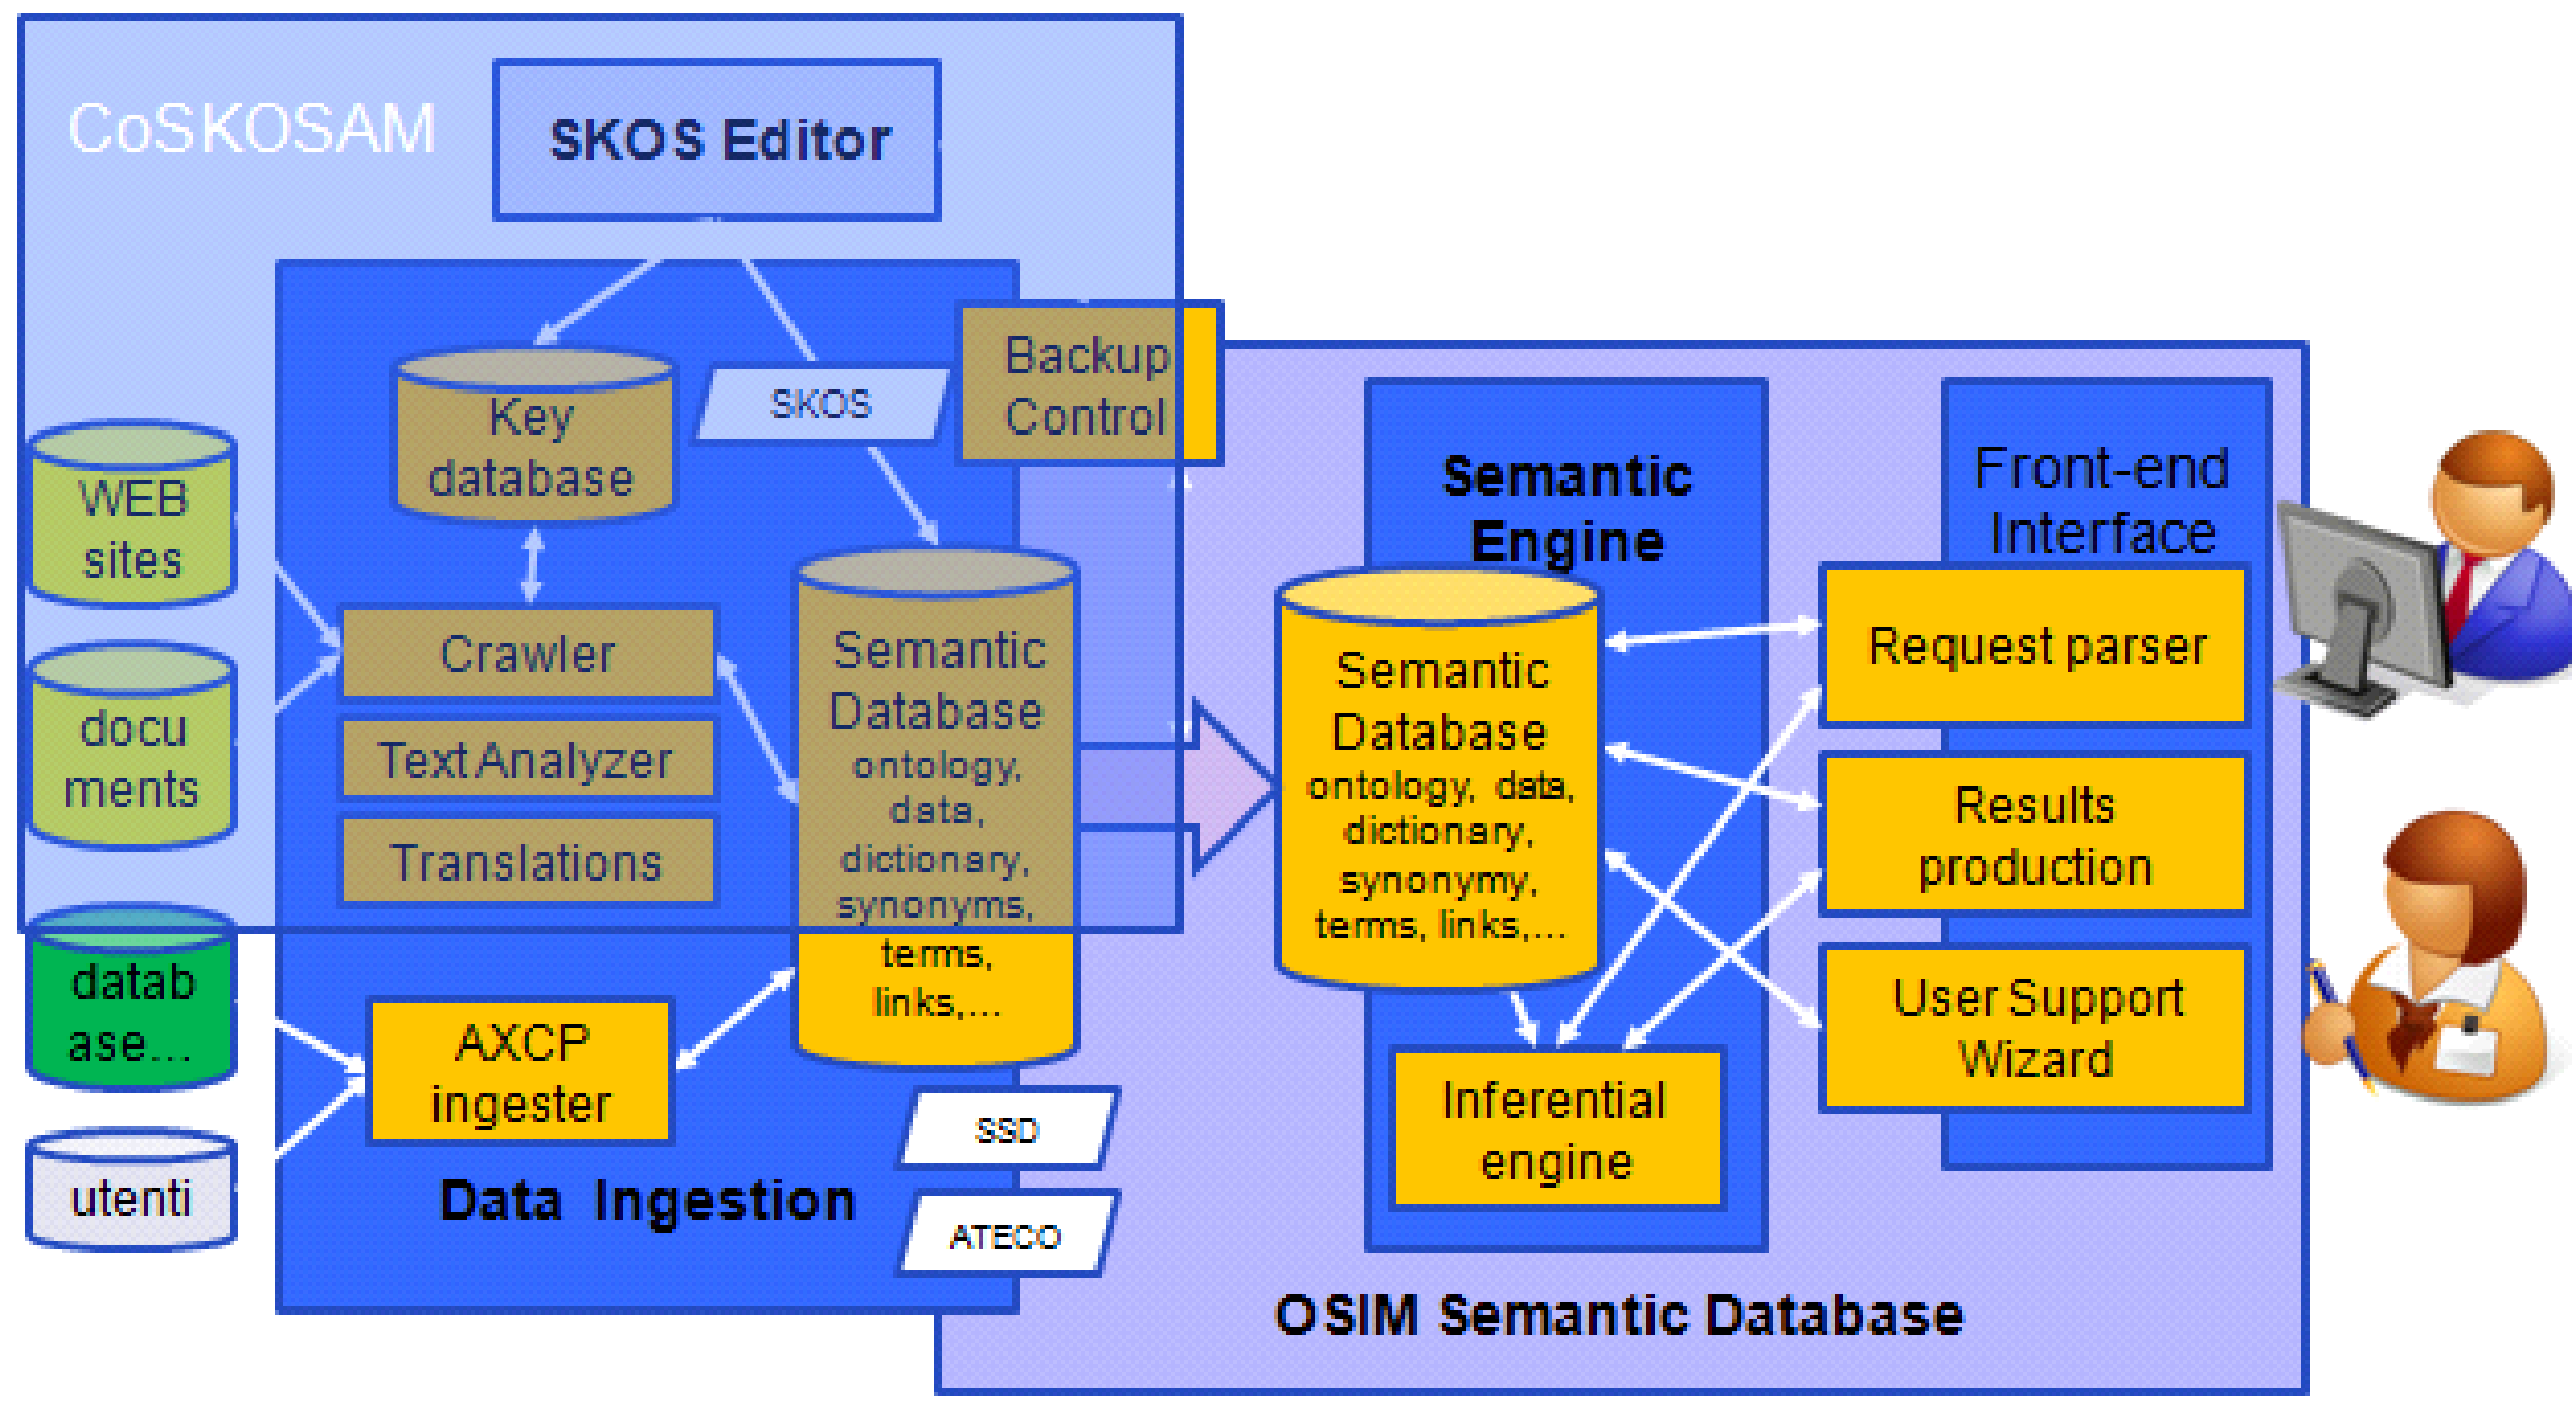
\includegraphics[height=0.5\textheight]{img/schemaOsim}
    \end{center}
  \end{block}
  \pause
  \begin{itemize}
  \item Creare una \alert{base di conoscenza} del personale universitario
    \pause
  \item Organizzare le \alert{competenze} in modo \alert{gerarchico}
    \pause
  \item Possibilit\`a di effettuare \alert{query}
  \end{itemize}
\end{frame}

\begin{frame}{Problema specifico}
  \begin{block}{Collaborative SKOS Accelerator and Manager}
    \makebox[\textwidth][c]{
  \begin{tikzpicture}[auto]
    \node [weblist, font = \dimg, minimum width = 1.5cm, minimum height = 1cm] (web) {Web};
    \node [app2, right = 1.5cm of web, font = \dimg, minimum width = 2cm] (crawler) {Crawler};
    \draw [freccia] (web) -- (crawler);

    \node [db, above = 0.5cm of crawler, font = \dimg] (keydb) {Keyword};
    \draw [dfreccia] (keydb) -- (crawler);

    \node [app3, below = 0.1cm of crawler, font = \dimg, minimum width = 1.75cm] (textana) {Analisi testo};
    \node [app3, below = 0.1cm of textana, font = \dimg, minimum width = 1.75cm] (trad) {Traduzioni};

    \node [rdf, right = 3cm of crawler, font = \dimg] (rdf) {Base\\di\\conoscenza};
    \draw [freccia] (crawler) -- (rdf);

    \node [app, right = 1cm of keydb, font =\dimg] (editor) {Editor};
    \draw [dfreccia] (editor) -- (keydb);
    \draw [dfreccia] (editor) -- (rdf);
  \end{tikzpicture}
}

  \end{block}
  \begin{itemize}
  \item Il lavoro si concentra su \alert{CoSKOSAM}, in particolar modo sul \alert{crawler}
    \pause
  \item Il crawler si presentava destrutturato e non funzionante
    \pause
  \item Le pagine da acquisire presentano una struttura complessa,\\
    cos\`i come l'ontologia su cui scrivere
    \pause
  \item \`E stato svolto un lavoro di \alert{studio} del progetto
    \pause
  \item Sono state implementate \alert{nuove funzionalit\`a}
  \end{itemize}
\end{frame}

\subsection{Strutture usate}

\begin{frame}{Strutture usate}
  \begin{itemize}
  \item Vengono usate le strutture semantiche \alert{RDF}, \alert{RDFS}, \alert{OWL}\\
    per la memorizzazione dell'informazioni
    \pause
  \item Viene usato il \alert{framework GATE} per l'analisi del linguaggio naturale
    \pause
  \item Vengono usate l'ontologia \alert{SKOS} e \alert{FOAF}\\
    per rappresentare competenze e persone 
  \end{itemize}
\end{frame}

\section{Lavoro svolto}

\subsection{Ontologia}

\begin{frame}{Scrittura nell'ontologia}
  \makebox[\textwidth][c]{
  \begin{tikzpicture}[auto]
    \matrix[row sep = 0.5cm, column sep = 2cm] {
      %prima
      \uncover<1->{\node[uri] (persona) {\dimt \alert<1-5,9,13>{Persona}};}\pgfmatrixnextcell
      \uncover<13->{\node[uri] (bnode) {};}\\
      %seconda
      \uncover<6->{\node[uri] (insegnamento) {\dimt \alert<6-9,14>{Insegnam.}};}\pgfmatrixnextcell
      \uncover<10->{\node[uri] (competenza) {\dimt \alert<10-14>{Compet.}};}\\
    };
    \begin{scope}[node distance = 2cm]
      %nodi di persona
      \uncover<4->{\node[uriEsistente, left = 2.3cm of persona] (dipartimento) {\dimt \alert<4>{Dipart.}};}
      \uncover<1->{\node[uriEsistente, above left = 0.6cm and 1.5cm  of persona] (classePers) {\codt{\alert<1>{foaf:Person}}};}
      \uncover<2->{\node[uriChoice, above left = 1.3cm and 0cm of persona] (classiPers) {
        \codt{\alert<2>{uni:AssociateProfessor}}\\
        \codt{\alert<2>{uni:Professor}}\\
        \codt{\alert<2>{uni:FullResearcher}}
        %\codt{uni:Researcher}
      };}
      \uncover<3->{\node[letterale, above = of persona] (nomePers) {\dimt \alert<3>{Nome}};}
      \uncover<5->{\node[letterale, above right = 2cm and 1cm of persona] (url1Pers) {\dimt \alert<5>{Url}};}
      \uncover<5->{\node[letterale, above right = 1.2cm and 2.4cm of persona] (url2Pers) {\dimt \alert<5>{Url}};}

      %nodi di bnode
      \uncover<13->{\node[letterale, above right = 2.5cm of bnode] (occorrenze) {\dimt \alert<13>{Occorrenze}};}
      
      %nodi di insegnamento
      \uncover<6->{\node[uriEsistente, left = 1.5cm of insegnamento] (classeIns) {\codt{\alert<6>{uni:Course}}};}
      \uncover<7->{\node[letterale, below left = of insegnamento] (nomeIns) {\dimt \alert<7>{Nome}};}
      \uncover<8->{\node[letterale, below = of insegnamento] (urlIns) {\dimt \alert<8>{Url}};}

      %nodi di competenza
      \uncover<10->{\node[uriEsistente, below right = of competenza] (classeComp) {\codt{\alert<10>{skos:concept}}};}
      \uncover<12->{\node[uriEsistente, below = 1.8cm of competenza] (altraClasseComp) {\codt{\alert<12>{uni:temporaryXXXStore}}};}
      \uncover<11->{\node[letterale, right = of competenza] (nomeComp) {\dimt \alert<11>{Nome}};}
    \end{scope}

    %frecce persona
    \uncover<9->{\draw[ufreccia] (persona) to node[labelog]{\codt{\alert<9>{uni:takeCourse}}} (insegnamento);}
    \uncover<4->{\draw[freccia] (persona) to node[labelg]{\codt{\alert<4>{uni:isAffiliatedOf}}} (dipartimento);}
    \uncover<1->{\draw[freccia] (persona) to node[labelg]{\codt{\alert<1>{rdf:type}}} (classePers);}
    \uncover<2->{\draw[tfreccia] (persona) to node[labelg]{\codt{\alert<2>{rdf:type}}} (classiPers);}
    \uncover<3->{\draw[freccia] (persona) to node[labelg]{\codt{\alert<3>{foaf:name}}} (nomePers);}
    \uncover<5->{\draw[freccia] (persona) to node[labelg]{\codt{\alert<5>{uni:hasPageUrl}}} (url1Pers);}
    \uncover<5->{\draw[freccia] (persona) to node[labelg]{\codt{\alert<5>{uni:hasSecondPageUrl}}} (url2Pers);}
    \uncover<13->{\draw[ufreccia] (persona) to node[labelg]{\codt{\alert<13>{uni:hasCompetence}}} (bnode);}

    %frecce bnode
    \uncover<13->{\draw[freccia] (bnode) to node[labelg]{\codt{\alert<13>{uni:hasOccurrence}}} (occorrenze);}
    \uncover<13->{\draw[freccia] (bnode) to node[labelog]{\codt{\alert<13>{uni:competenceType}}} (competenza);}


    %frecce insegnamento
    \uncover<6->{\draw[freccia] (insegnamento) to node[labelg]{\codt{\alert<6>{rdf:type}}} (classeIns);}
    \uncover<14->{\draw[tufreccia] (insegnamento) to node[labelg, below]{\codt{\alert<14>{skos:subject}}} (competenza);}
    \uncover<7->{\draw[freccia] (insegnamento) to node[labelg]{\codt{\alert<7>{rdfs:label}}} (nomeIns);}
    \uncover<8->{\draw[freccia] (insegnamento) to node[labelg]{\codt{\alert<8>{uni:hasPageUrl}}} (urlIns);}

    %frecce competenza
    \uncover<12->{\draw[tfreccia] (competenza) to node[labelg]{\codt{\alert<12>{rdf:type}}} (altraClasseComp);}
    \uncover<10->{\draw[freccia] (competenza) to node[labelg]{\codt{\alert<10>{rdf:type}}} (classeComp);}
    \uncover<11->{\draw[freccia] (competenza) to node[labelg]{\codt{\alert<11>{skos:prefLabel}}} (nomeComp);}
  \end{tikzpicture}
}

\end{frame}

\begin{frame}{Creazione dello SKOS}
  \begin{columns}
    \begin{column}{5cm}
      \makebox[\textwidth][c]{
  \begin{tikzpicture}[auto]
    \node[uri] (comp) {\dimt Competenza};
    \visible<2>{\node[uriEsistente, below = 1.8cm of comp] (schema) {\dimt Concept schema};}
    \visible<3>{\node[uriEsistente, below = 1.5 of comp] (altra) {\dimt Competenza};}
    
    %nodi di comp
    \node[uriEsistente, above left = 1.5cm and 0.5cm of comp.north] (tipoComp) {\codt{skos:Concept}};
    \node[letterale, above right = 1.7cm and 0.5cm of comp.north] (nomeComp) {\dimt Nome};
    
    %nodi di schema
    \visible<2>{\node[uriEsistente, below = 1.2cm of schema] (tipoSchema) {\codt{skos:ConceptScheme}};}

    %nodi di altra
    \visible<3>{\node[uriEsistente, below left = 1.5cm and 0.5cm of altra.south] (tipoAltra) {\codt{skos:Concept}};}
    \visible<3>{\node[letterale, below right = 1.7cm and 0.5cm of altra.south] (nomeAltra) {\dimt Nome};}
      
    
    %frecce comp
    \draw[freccia] (comp) to node[labelg]{\codt{rdfType}} (tipoComp);
    \draw[freccia] (comp) to node[labelg]{\codt{skos:prefLabel}} (nomeComp);

    %frecce schema
    \visible<2>{\draw[freccia] (schema) to node[labelg, align = left, font = \dimt]{skos:\\hasTopConcept} (comp);}
    \visible<2>{\draw[freccia] (schema) to node[labelg]{\codt{rdfType}} (tipoSchema);}

    %frecce altra
    \visible<3>{\draw[freccia] (altra) to node[labelg]{\codt{skos:narrower}} (comp);}
    \visible<3>{\draw[freccia] (altra) to node[labelg]{\codt{rdfType}} (tipoAltra);}
    \visible<3>{\draw[freccia] (altra) to node[labelg]{\codt{skos:prefLabel}} (nomeAltra);}

  \end{tikzpicture}
}

    \end{column}
    \begin{column}{5cm}
      \begin{itemize}
        \item Interviene\\
          l'\alert{esperto di dominio}\\
          per la creazione\\
          dello \alert{SKOS}
          \pause
        \item La competenza\\
          pu\`o essere inserita\\
          come \alert{radice} dello SKOS
          \pause
        \item Oppure\\
          come \alert{specificazione}\\
          di un'altra competenza
      \end{itemize}
    \end{column}
  \end{columns}
\end{frame}

\subsection{Crawler keyword}

\begin{frame}{Crawler keyword}{Problemi principali}
  \begin{itemize}
  \item Reperire tutte le pagine del dipartimento\\
    seguendo una \alert{struttura complessa}
    \pause
  \item \`E necessario del \alert{NLP} per individuare nel testo le \alert{keyword}
    \pause
  \item Gestire i casi in cui le keyword siano di \alert{lingue diverse}
    \pause
  \item Va gestito il caso in cui l'estrazione delle keyword dia \alert{esiti errati}
  \end{itemize}
\end{frame}

\begin{frame}{Schema crawling keyword}
  \makebox[\textwidth][c]{
  \begin{tikzpicture}[auto]
    \node [db] (tabDip) {\dimg Dipartimenti};
    \node [web, right = 0.5cm of tabDip] (listaPers) {\dimg Lista persone};
    \draw [freccia] (tabDip) -- (listaPers);
    \pause

    \node [gaz, above = 0.5cm of tabDip] (gazPers) {\dimg Gazetteer persone};
    \node [app, right = 0.75cm of gazPers] (gate1) {\dimg Estr. \emph{link}};
    \node [weblist, right = 0.75cm of gate1] (pagine) {\dimg \emph{url} pagine};
    \node [gate, below = 1cm of pagine] (gate) {\dimg GATE};
    \draw [freccia] (listaPers) -- (gate1);
    \draw [freccia] (gazPers) -- (gate1);
    \draw [freccia] (gate1) -- (pagine);
    \draw [dfreccia] (gate) -- (gate1);
    \pause

    \node [app, right = 0.75cm of pagine] (gate2) {\dimg Estr. frasi};
    \node [filelist, below = 1cm of gate2] (files) {\dimg File frasi};
    \draw [freccia] (pagine) -- (gate2);
    \draw [freccia] (gate2) -- (files);
    \draw [dfreccia] (gate) -- (gate2);
    \pause

    \node [app, below = 1.5cm of files] (gate3) {\dimg Ricon. lingua};
    \node [file, left = 0.75cm of gate3] (fileEn) {\dimg Frasi ing.};
    \node [file, above = 0.25cm of fileEn] (fileIt) {\dimg Frasi ita.};
    \node [file, below = 0.25cm of fileEn] (fileBo) {\dimg Frasi scon.};
    \draw [freccia] (files) -- (gate3);
    \draw [freccia] (gate3) -- (fileIt);
    \draw [freccia] (gate3) -- (fileEn);
    \draw [freccia] (gate3) -- (fileBo);
    \draw [dfreccia] (gate) -- (gate3);
    \pause

    \node [app, left = 0.75cm of fileEn] (gate4) {\dimg Estr. sostantivi};
    \node [gaz, above left = 0.5cm and 0.5cm of gate4.north] (gazStop) {\dimg Stop words};
    \node [tab, left = 0.75cm of gate4] (keytab) {\dimg Tabella};
    \draw [freccia] (fileIt) -- (gate4);
    \draw [freccia] (fileEn) -- (gate4);
    \draw [freccia] (gazStop) -- (gate4);
    \draw [freccia] (gate4) -- (keytab);
    \draw [dfreccia] (gate) -- (gate4);
    \pause

    \node [app, below = 0.5cm of keytab] (trad) {\dimg Traduz.};
    \node [db, right = 0.75cm of trad] (cache) {\dimg Cache};
    \node [webapp, below right = 0.25cm and 1cm of trad] (google) {\dimg Google};
    \node [db, below = 0.5cm of trad] (keydbtab) {\dimg \emph{Keyword}};  
    \draw [freccia] (keytab) -- (trad);
    \draw [dfreccia] (cache) -- (trad);
    \draw [dfreccia] (google) -- (trad);
    \draw [freccia] (trad) -- (keydbtab);  
  \end{tikzpicture}
}

\end{frame}

\subsection{Crawler competenze}

\begin{frame}{Crawler competenze}{Problemi principali}
  \begin{itemize}
  \item Reperire le pagine di ogni persona
    \pause
  \item Individuare le \alert{competenze} associate alle persone
    \pause
  \item Reperire la \alert{struttura} (persone, corsi, dipartimenti) dalle pagine
    \pause
  \item Scrivere le informazioni nell'\alert{ontologia}
    \pause
  \item Va gestito il \alert{multilingua} delle competenze
  \end{itemize}
\end{frame}

\begin{frame}{Schema crawling competenze}
  \makebox[\textwidth][c]{
  \begin{tikzpicture}[auto]
    \node [db] (tabDip) {\dimg Dipartimenti};
    \node [web, right = 0.5cm of tabDip] (listaPers) {\dimg Lista persone};
    \draw [freccia] (tabDip) -- (listaPers);
    \pause

    \node [gaz, above = 1cm of tabDip] (gazPers) {\dimg Gazetteer persone};
    \node [app, right = 1cm of gazPers] (estr) {\dimg Estr. \emph{link}};
    \node [tab, right = 1cm of estr] (tabella) {\dimg Tabella};
    \node [gate, below = 0.75cm of estr.east] (gate) {\dimg GATE};
    \draw [freccia] (listaPers) -- (estr);
    \draw [freccia] (gazPers) -- (estr);
    \draw [freccia] (estr) -- (tabella);
    \draw [dfreccia] (estr) -- (gate);
    \pause

    \node [round, below = 0.5cm of tabella] (pallino) {};
    \node [app, below = 0.5cm of pallino] (analisi) {\dimg Analisi pers.};
    \node [app, below right = 0.5cm and 1cm of analisi.south] (trad) {\dimg Traduz.};
    \node [db, right = 0.75cm of analisi] (carriera) {\dimg Carriera};
    \node [rdfclist, below = 1.5cm of analisi] (insegnamenti) {\dimg Istanze\\\dimg insegn.};
    \node [rdfc, left = 0.5cm of insegnamenti] (persona) {\dimg Istanza\\\dimg persona};
    \node [rdfclist, right = 0.5cm of insegnamenti] (competenze) {\dimg Istanze\\\dimg compet.};
    \draw [freccia] (tabella) -- (pallino);
    \draw [freccia] (pallino) -- (analisi);
    \draw [freccia] (carriera) -- (analisi);
    \draw [freccia] (analisi) -- (persona);
    \draw [freccia] (analisi) -- (insegnamenti);
    \draw [freccia] (analisi) -- (trad);
    \draw [freccia] (trad) -- (competenze);
    \draw [dfreccia] (analisi) -- (gate);
    \pause

    \node [app, below = 0.75cm of insegnamenti] (serializza) {\dimg Serializ.};
    \node [rdf, left = 1cm of serializza] (rdf) {\dimg RDF store};
    \draw [freccia] (persona) -- (serializza);
    \draw [freccia] (insegnamenti) -- (serializza);
    \draw [freccia] (competenze) -- (serializza);
    \draw [freccia] (serializza) -- (rdf);
    \pause

    \node [choice, vuoto, right = 0.5cm of serializza] (rombo) {};
    \node [point, right = 0.25cm of carriera] (p) {};
    \draw [freccia] (serializza) -- (rombo);
    \draw [nfreccia] (rombo) -| (p);
    \draw [freccia] (p) |- (pallino);
  \end{tikzpicture}
}

\end{frame}

\subsection{Dettagli progettuali}

\begin{frame}{Servlet}
  \begin{block}{schema}
    \makebox[\textwidth][c]{
    \begin{tikzpicture}[auto]
      \node [web] (jsp) {Pagina \emph{JSP}};
      \node [app2, right = 2cm of jsp] (servlet) {Servlet};
      \node [app2, below = 1.5cm of servlet] (factory) {Command factory};
      \node [app2, right = 2cm of servlet] (gestore) {Gestore comandi};
      \node [app2, below = 1.5cm of gestore] (altro) {Eventuali altri oggetti};
      
      \draw [dfreccia] (jsp) -- (servlet);
      \draw [dfreccia] (servlet) -- (factory);
      \draw [dfreccia] (servlet) -- (gestore);
      \draw [dtfreccia] (gestore) -- (altro);
      
      %evidenzia
      \visible<2>{\draw [evidenzia, xscale=2.5] (jsp) circle (0.5cm);}
      \visible<3>{\draw [evidenzia, xscale=1.75] (servlet) circle (0.5cm);}
      \visible<4>{\draw [evidenzia, xscale=3.5] (factory) circle (0.5cm);}
      \visible<5>{\node [evidenziaRett, on grid, below = 1.1cm of gestore, text width = 3.75cm, text height = 2.75cm] {};}
      \node[point, above = 0.25cm of gestore.north west] (p1) {};
      \node[point, above = 0.25cm of jsp.north east] (p2) {};
      \visible<6>{\draw [evidenziaFrecc] (p1) -- (p2);}
    \end{tikzpicture}
}

  \end{block}
  \pause
  \begin{itemize}
    \item Pagine \alert{JSP}
      \pause
    \item Chiamate \alert{HTTP} tramite \alert{Javascript} alla \alert{Servlet}
      \pause
    \item Creazione \alert{gestore comandi}
      \pause
    \item Esecuzione comando
      \pause
    \item Risposta \alert{JSON} alla pagina
  \end{itemize}
\end{frame}

\begin{frame}{Dettagli crawler}
  \begin{block}{schema}
    \makebox[\textwidth][c]{
  \begin{tikzpicture}[auto]
    \node [app2] (gest) {\dimg Gestore\\\dimg comandi};

    \node [coda, right = 0.5cm of gest] (coda) {\dimg Coda\nodepart{two}\dimg processi};
    \node [point, above left = 0.5cm and 0.25cm of coda] (p1) {};
    \node [point, below right = 0.5cm and 0.25cm of coda] (p2) {};

    \node [app2, right = 0.5cm of coda] (thread) {\dimg Thread};
    \node [choice, vuoto, right = 0.5cm of thread] (cho) {};

    \node [app2, above right = 0.25cm and 0.5cm of cho.east, text width=2.5cm] (keyeng) {\dimg Keyword engine};
    \node [app2, below right = 0.25cm and 0.5cm of cho.east, text width=2.5cm] (coeng) {\dimg Competence engine};

    \node [app3, above = 0.5cm of keyeng] (landet) {\dimg Language detector};
    \node [app3, left = 0.5cm of landet] (chuspli) {\dimg Chunk splitter};
    \node [app4, right = 0.5cm of landet] (keyman) {\dimg Keyword Manager};

    \node [point, above = 0.3cm of landet] (p3) {};
    \node [point, right = 4.5cm of p3] (p4) {};
    \node [point, below = 1.25cm of p4] (p5) {};

    \node [app3, right = 4cm of cho] (gate) {\dimg Gate};

    \node [app3, below = 0.5cm of coeng, xshift = 0.5cm] (pan) {\dimg Person analyzer};
    \node [app4, right = 0.5cm of pan] (rdf) {\dimg RDF serializer};
    \node [app3, left = 0.7cm of pan] (ois) {\dimg Ontology instance};

    \node [point, below = 0.3cm of pan] (p6) {};
    \node [point, right = 4cm of p6] (p7) {};
    \node [point, above = 1.25cm of p7] (p8) {};

    \draw [freccia] (gest.east) -| (p1) -| (coda.north);
    \draw [freccia] (coda.south) |- (p2) |- (thread.west);
    \draw [freccia] (thread) -- (cho);
    \draw [freccia] (cho) |- (keyeng);
    \draw [freccia] (cho) |- (coeng);

    \draw [dfreccia] (keyeng) -- (chuspli);
    \draw [dfreccia] (keyeng) -- (landet);
    \draw [freccia] (keyeng) -- (keyman);

    \draw [dfreccia] (coeng) -- (pan);
    \draw [dfreccia] (pan) -- (ois);
    \draw [freccia] (coeng) -- (rdf);

    \draw [dfreccia] (keyeng.east) -- (gate);
    \draw [dfreccia] (coeng.east) -- (gate);

    \draw [nfreccia] (p3) -- (p4);
    \draw [nfreccia] (p4) -- (p5);
    \draw [freccia] (p5) -- (gate);
    \draw [freccia] (p3) -- (landet);
    \draw [freccia] (p3) -| (chuspli);

    \draw [nfreccia] (p6) -- (p7);
    \draw [nfreccia] (p7) -- (p8);
    \draw [freccia] (p6) -- (pan);
    \draw [freccia] (p8) -- (gate);

    \draw<2> [evidenzia, yscale=1.5] (coda) circle (1cm);
    \draw<3> [evidenzia, xscale=1.5] (thread) circle (0.5cm);
    \node[point, right = 1.5cm of cho] (pe) {};
    \draw<4> [evidenzia, xscale=2] (pe) circle (1.2cm);
  \end{tikzpicture}
}

  \end{block}
  \pause
  \begin{itemize}
    \item Viene usata una \alert{coda di processi}
      \pause
    \item Sequenzialmente viene creato un \alert{thread} per ogni processo della coda
      \pause
    \item Il thread chiama il giusto \alert{engine} secondo l'operazione richiesta
      \pause
  \end{itemize}
\end{frame}

\section{Conclusioni}

\subsection{Interfaccia}

\begin{frame}{Interfaccia keyword}
  \begin{columns}
    \begin{column}{0.5\textwidth}
      
\includegraphics[width=\textwidth]{img/pannelloAmministrazione2}
    \end{column}
    \begin{column}{0.5\textwidth}
      \begin{itemize}
      \item Interviene un \alert{esperto di dominio}
        \pause
      \item Sceglie quali sono le \alert{keyword} significative
        \pause
      \item Le keyword scelte sono inserite in un \alert{gazetteer}
      \end{itemize}
    \end{column}
  \end{columns}
\end{frame}

\begin{frame}{Interfaccia SKOS}
%  \begin{textblock*}{12.8cm}(0cm,0cm)
%    %pulsanti
\tikz[baseline, overlay]\node[point] (pp) at (2.5cm,7.5cm){};
\tikz[baseline, overlay]\draw<2> [evidenzia, xscale=4] (pp) circle (0.3cm);

%tab
\tikz[baseline, overlay]\node[point] (pt) at (2.7cm,8.25cm){};
\tikz[baseline, overlay]\draw<3> [evidenzia, xscale=6] (pt) circle (0.3cm);

%lingua
\tikz[baseline, overlay]\node[point] (pl) at (10cm,8.9cm){};
\tikz[baseline, overlay]\draw<4> [evidenzia, xscale=1.5] (pl) circle (0.4cm);

%skos
\tikz[baseline, overlay]\node[point] (ps) at (6cm,6.6cm){};
\tikz[baseline, overlay]\draw<5> [evidenzia, xscale=2] (ps) circle (3cm);

%log
\tikz[baseline, overlay]\node[point] (pl) at (3.35cm,4cm){};
\tikz[baseline, overlay]\draw<6> [evidenzia, xscale=1.5] (pl) circle (1.5cm);

%processi
\tikz[baseline, overlay]\node[point] (ppr) at (7.7cm,4.5cm){};
\tikz[baseline, overlay]\draw<7> [evidenzia, xscale=2.2] (ppr) circle (1.5cm);

%  \end{textblock*}
  \begin{center}
    
\includegraphics[height=0.8\textheight]{img/pannelloAmministrazione1}
  \end{center}
  %pulsanti
\tikz[baseline, overlay]\node[point] (pp) at (2.5cm,7.5cm){};
\tikz[baseline, overlay]\draw<2> [evidenzia, xscale=4] (pp) circle (0.3cm);

%tab
\tikz[baseline, overlay]\node[point] (pt) at (2.7cm,8.25cm){};
\tikz[baseline, overlay]\draw<3> [evidenzia, xscale=6] (pt) circle (0.3cm);

%lingua
\tikz[baseline, overlay]\node[point] (pl) at (10cm,8.9cm){};
\tikz[baseline, overlay]\draw<4> [evidenzia, xscale=1.5] (pl) circle (0.4cm);

%skos
\tikz[baseline, overlay]\node[point] (ps) at (6cm,6.6cm){};
\tikz[baseline, overlay]\draw<5> [evidenzia, xscale=2] (ps) circle (3cm);

%log
\tikz[baseline, overlay]\node[point] (pl) at (3.35cm,4cm){};
\tikz[baseline, overlay]\draw<6> [evidenzia, xscale=1.5] (pl) circle (1.5cm);

%processi
\tikz[baseline, overlay]\node[point] (ppr) at (7.7cm,4.5cm){};
\tikz[baseline, overlay]\draw<7> [evidenzia, xscale=2.2] (ppr) circle (1.5cm);

\end{frame}

\subsection{Risultati}

\begin{frame}{Risultati}
  \begin{columns}
    \begin{column}{0.3\textwidth}
      Sono stati acquisiti:
    \end{column}
    \begin{column}{0.35\textwidth}
      \begin{itemize}
      \item  \alert{49} dipartimenti
      \item  \alert{249000} keyword
      \end{itemize}
    \end{column}
    \begin{column}{0.35\textwidth}
      \begin{itemize}
      \item  \alert{13000} documenti
      \item  \alert{2344} docenti
      \end{itemize}
    \end{column}
  \end{columns}
  \pause
  \vspace{0.5cm}
  Stato dei principali dipartimenti per i quali \`e stata fatta la \alert{validazione}:
  \begin{tabular}{|p{8cm}|r|r|r|}
    \hline 
    \textbf{Dipartimento} & \textbf{Key.} & \textbf{Gaz.} & \textbf{Doc.} \\
    \hline 
    Dipartimento di meccanica & 2958 & 523 & 92 \\
    \hline
    Dipartimento di Anat., Ist. e Medicina Legale & 2012 & 909 & 400\\
    \hline
    Dipartimento di Elettronica e Telecomunicazioni & 6660 & 430 & 255\\
    \hline
    Dipartimento di Ingegneria Civile e Ambientale & 6502 & 470 & 245\\
    \hline
    Dipartimento di Scienze della Terra & 10127 & 143 & 179\\
    \hline
    Dipartimento di Teoria e Storia del Diritto & 6574 & 1173 & 43\\
    \hline
    Dipartimento di scienze economiche & 5115 & 1047 & 285\\
    \hline
    Dipartimento di matematica per le decisioni & 2258 & 232 & 122\\
    \hline
    Dipartimento di sistemi ed informatica & 7803 & 1733 & 335\\
    \hline
  \end{tabular}
\end{frame}

\begin{frame}{Conclusioni}
  \begin{itemize}
  \item Sono stati studiati ed analizzati il \alert{problema} e le diverse \alert{complessit\`a}
    \pause
  \item I problemi principali sono la \alert{struttura delle pagine},\\
    creare una \alert{ontologia} che possa essere amministrata e interrogata\\
    e fornire una \alert{interfaccia} usabile
    \pause
  \item Sono state formulate e implementate le due fasi di crawling
    \pause
  \item Sono stati proposti possibili \alert{sviluppi futuri}, ad esempio
    \begin{itemize}
    \item usare \alert{XSLT} per implementare una fase di pre-crawling
    \item identificare le keyword anche con i \alert{verbi}
    \item un miglioramento della parte di query sull'ontologia
    \end{itemize}
  \end{itemize}
\end{frame}

\section*{}

\begin{frame}
  \begin{center}
    $\mathcal{FINE}$
  \end{center}
\end{frame}

\appendix

\section{\appendixname}

\begin{frame}{Rappresentazioni semantiche}{RDF, RDFS, OWL}
  \begin{itemize}
  \item \alert{RDF} permette di rappresentare:\\
    \alert{risorse}, \alert{asserzioni} su di esse e relazioni tra di esse
    \pause
    \begin{itemize}
    \item Le risorse sono identificate univocamente da \alert{URI}
      \pause
    \item Le asserzioni sono rappresentate da \alert{triple}:\\
      \alert{soggetto} - \alert{predicato} - \alert{oggetto}
      \pause  
    \end{itemize}
  \item \alert{RDFS} \`e una estenzione semantica di RDF che fornisce\\
    un vocabolario per definire \alert{classi} e \alert{propriet\`a}
    \pause
    \begin{itemize}
    \item Le risorse possono essere divise in classi, i membri delle classi\\
      sono dette \alert{istanze} e vengono definite tramite \texttt{rdf:type}
      \pause
    \item \`E possibile definire \alert{sottoclassi} tramite \texttt{rdfs:subClassOf}
      \pause
    \item \`E possibile definire \alert{sottopropriet\`a} tramite \texttt{rdfs:subPropertyOf}
      \pause
    \item \`E possibile definire un \alert{dominio} di una propriet\`a\\
      con \texttt{rdfs:domain} e un'\alert{immagine} con \texttt{rdfs:range}
      \pause
    \end{itemize}
  \item \alert{OWL} estende RDFS per creare strutture logiche
    \pause
    \begin{itemize}
    \item Le strutture descritte con OWL si chiamano \alert{ontologie}
      \pause
    \item Sulle ontologie \`e possibile estrarre conoscenza con dei \alert{reasoner}
    \end{itemize}
  \end{itemize}
\end{frame}

\begin{frame}{Framework GATE}{General Architecture for Text Engineering}
  \begin{itemize}
  \item \`E un framework open source per lo sviluppo di applicazioni\\
    per l'analisi del linguaggio naturale
    \pause
  \item Fornisce un editor di sviluppo \alert{GATE Developer}\\
    e una API \alert{GATE Embedded}
    \pause
  \item Le applicazione sono costituite da \alert{plugin}\\
    eseguiti in cascata sui documenti
    \pause
  \item I plugin creano delle \alert{annotazioni} sui documenti
    \pause
  \item I \alert{gazetteer} sono insiemi di liste di parole che vengono annotate
    \pause
  \item Le regole \alert{JAPE} permettono di individuare pattern nelle annotazioni\\
    utilizzando espressioni regolari
    \pause
  \item \alert{ANNIE} \`e una pipeline che annota nel testo parole, frasi,\\
    e parti del testo (sostantivi, verbi, etc\dots)
  \end{itemize}
\end{frame}

\begin{frame}{RDF}{Resource Description Framework}
  \begin{itemize}
  \item Rappresentare \alert{risorse}, \alert{asserzioni} su di esse e relazioni tra di esse
    \pause
  \item Le risorse sono identificate univocamente da \alert{URI}
    \pause
  \item Le asserzioni sono rappresentate da \alert{triple}
    \pause
    \begin{itemize}
    \item Il \alert{soggetto} deve essere un URI
      \pause
    \item Il \alert{predicato} deve essere un URI
      \pause
    \item L'\alert{oggetto} pu\`o essere un URI o un letterale
      \pause
    \end{itemize}
  \item Possibilit\`a di usare \alert{blank node} per i soggetti e oggetti
    \pause
  \item Possibilit\`a di usare la \alert{reificazione}\\
    per fare asserzioni su di una asserzione
  \end{itemize}
\end{frame}

\begin{frame}{RDFS}{RDF Schema}
  \begin{itemize}
  \item Estenzione semantica di RDF che fornisce un vocabolario\\
    per definire \alert{classi} e \alert{propriet\`a}
    \pause
  \item Le risorse possono essere divise in classi, i membri delle classi\\
    sono dette \alert{istanze} e vengono definite tramite \texttt{rdf:type}
    \pause
  \item \`E possibile definire \alert{sottoclassi} tramite \texttt{rdfs:subClassOf}
    \pause
  \item Le propriet\`a sono i predicati di RDF
    \pause
  \item \`E possibile definire \alert{sottopropriet\`a} tramite \texttt{rdfs:subPropertyOf}
    \pause
  \item \`E possibile definire un \alert{dominio} di una propriet\`a\\
    con \texttt{rdfs:domain} e un'\alert{immagine} con \texttt{rdfs:range}
    \pause
  \item Esistono dei vocabolari per definire \alert{contenitori} e \alert{collezioni}
  \end{itemize}
\end{frame}

\begin{frame}{OWL}{Web Ontology Language}
  \begin{itemize}
  \item Estende RDFS per creare strutture logiche
    \pause
  \item Le strutture descritte con OWL si chiamano \alert{ontologie}
    \pause
  \item Sulle ontologie \`e possibile estrarre conoscenza con dei \alert{reasoner}
    \pause
  \item Esistono tre dialetti con livelli di espressivit\`a logica crescenti
  \end{itemize}
\end{frame}

\begin{frame}{SKOS}{Simple Knowledge Organization System}
  \begin{itemize}
  \item \`E un vocabolario RDF che permette\\
    la descrizione di sistemi di organizzazione
    \pause
  \item L'elemento fondamentale \`e il \alert{concept}\\
    definito come istanza di \texttt{skos:Concept}
    \pause
  \item Si indicano le label con:\\
    \texttt{skos:prefLabel}, \texttt{skos:altLabel}, \texttt{skos:hiddenLabel}
    \pause
  \item Esistono \alert{relazioni semantiche} definite con:\\
    \texttt{skos:broader}, \texttt{skos:narrower} e \texttt{skos:relate}
    \pause
  \item I concept possono essere organizzati in \alert{vocabolari}\\
    istanze di \texttt{skos:ConceptScheme}\\
    con la propriet\`a \texttt{skos:inScheme}
  \end{itemize}
\end{frame}

\begin{frame}{FOAF}{Friend Of A Friend}
  \begin{itemize}
  \item \`E un vocabolario per definire una \alert{rete sociale} con RDF
    \pause
  \item La persona viene descritta come istanza di \texttt{foaf:Person}
    \pause
  \item La propriet\`a \texttt{foaf:name} specifica il nome di una persona
    \pause
  \item \texttt{foaf:knows} mette in relazione due persone
    \pause
  \item Esistono altre propriet\`a per indicare altri attributi di una persona,\\
    o per identificare l'appartenenza ad un gruppo
  \end{itemize}
\end{frame}
\end{document}
